Trois charges positives sont placées aux sommets d'un triangle rectangle : $q_1 = \qty{\v{q1}}{\micro\coulomb}$ au sommet de l'angle droit, $q_2 = \qty{\v{q2}}{\micro\coulomb}$ à \qty{\v{a}}{cm} à droite de $q_1$ et $q_3 = \qty{\v{q3}}{\micro\coulomb}$ à \qty{\v{b}}{cm} au-dessus de $q_1$.

\begin{center}
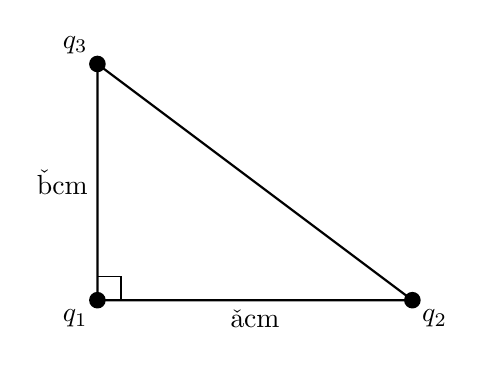
\begin{tikzpicture}
    \draw[thick] (0,0) -- (4,0) -- (0,3) -- cycle;
    \fill (0,0) circle (3pt) node[below left] {$q_1$};
    \fill (4,0) circle (3pt) node[below right] {$q_2$};
    \fill (0,3) circle (3pt) node[above left] {$q_3$};
    \node[below] at (2,0) {\qty{\v{a}}{cm}};
    \node[left] at (0,1.5) {\qty{\v{b}}{cm}};
    \draw (0,0.3) -- (0.3,0.3) -- (0.3,0);
\end{tikzpicture}
\end{center}

\begin{enumerate}[label=\alph*)]
    \item Déterminez le module de la force exercée sur $q_1$ par chacune des deux autres charges.
    \item Déterminez le module de la force résultante sur $q_1$.
    \item Déterminez l'orientation de la force résultante (angle par rapport à l'axe des $x$ négatifs).
\end{enumerate}
